\documentclass[10pt,twocolumn]{article}
\usepackage{amsmath}
\usepackage{graphicx}
\graphicspath{ {img/} }
\usepackage{geometry}
\geometry{left=3cm,right=3cm,top=3cm,bottom=3cm}
\usepackage{enumitem}
\usepackage{natbib}
\usepackage[symbol]{footmisc}
\renewcommand{\thefootnote}{\fnsymbol{footnote}}

\begin{document}
\title{CrankChain: Decentralized Asset Registration and Exchange}
\author{
{\normalsize Edward E. Kim}\\
\normalsize cranklin.com
}
\date{}

\maketitle
\subsection*{Abstract}
The author introduces CrankChain, a decentralized network for asset registration, and exchange.  CrankChain enables asset registration on the network and can be used to establish one's ownership of the asset with the added benefit of tokenization; assets can be distributed and exchanged as first-class members on-chain without relying on smart contracts, a virtual machine or state machine.  Furthermore, metadata pertaining to an asset can be appended to the asset's history by its owner(s).  CrankChain achieves this without sacrificing the simplicity nor the security of a single-dimensional blockchain.

\section{Introduction}
Many of the complaints surrounding \textit{Bitcoin} and other single-dimensional blockchains point towards the suboptimal transaction speed and cost\cite{wiki:btcscalability}.  While this makes it less than ideal for microtransactions, the benefits of this design is often overlooked.  \textit{Brewer's (CAP) Theorem}\cite{computer:brewercap} does not cease to exist in a decentralized datastore.  In fact, the boundaries are heightened.  Just as different centralized databases coexist with different strengths and weaknesses, so shall it be in decentralized networks.\\
In this paper, we introduce CrankChain which utilizes the many strengths of Satoshi Nakamoto's original design\cite{conf:nakamoto}.  By default, a decentralized network must be partition tolerant.  For the purposes of asset registration, tokenization, and exchange, we cannot sacrifice availability.  Consistency is important, but eventual consistency is sufficient.  Waiting for confirmation blocks will signal that the transaction is synchronized across a majority of nodes.  \\
CrankChain is designed under the philosophy that over-engineering opens the door to vulnerabilities.  By reducing the software's intrinsic complexity, open-source contributors are less likely to encounter surprises and improve upon the software's reliability and security.  For this reason, the software excludes a virtual machine, state machine, and support for smart contracts.  Though there are legitimate use cases for smart contracts\cite{whitepaper:buterin}, the use cases here do not require state changes per contract via transaction receipts\cite{yellow:wood}.  \\
The network strives to be truly decentralized.  It exists as a protocol.  The implementation can be used as a reference for future builds.  There is neither a gatekeeper to a permissioned network nor a central coordinator to route transactions.


\section{Protocol}
\subsection{Asset Transactions}
The tokenization of an arbitrary asset establishes its existence on the chain as if it were its own genesis block creation.  This is done by sending an \textit{ASSET\_CREATION} transaction. Forth, the token can be traded as a first-class member on-chain with \textit{STANDARD} transactions.  The native asset, Cranky Coin, is an asset just like any other tokenized asset on the network.  Its outlying property as the native asset is the fact that transaction fees and \textit{COINBASE} transactions are dealt in Cranky Coin.
All transactions include an asset type which defaults to the SHA256 sum of the string "Cranky Coin".  New assets can be registered by submitting a transaction with a \textit{ASSET\_CREATION} type enumerated value.  Hereinafter, the registrant owns that asset and may transact that asset though fees remain in the native asset type - Cranky Coin.
\subsection{Metadata}
Arbitrary metadata can be added to the chain via an \textit{ASSET\_ADDENDUM}  transaction.
Due to the nature of the blockchain's immutability, and infinite retention policy, all metadata addendums are appended and the history remains in tact.  CrankChain does not enforce a protocol for the metadata, but the author recommends using a protocol compatible with GNU diff\cite{man:diff}.
\subsection{**Exchange}
Asset owners are able to post a buy/sell limit order via \text{ORDER} transaction types.  Another transaction type, \textit{FILL}, allows for users to fill the posted limit order.  The limit order may also be cancelled by the original poster if the \textit{CANCEL} transaction is mined before a fill transaction.
\footnotetext[7]{future implementation}
\subsection{Peer Discovery}
When a new node joins the network, it queries all known nodes for its list of peers.  The node iterates over the known list of peers and initiates a handshake with each peer.  The handshake is initiated by requesting the peer's network configuration properties.  If the properties are identical to its own, it proceeds by sending a http POST request with a request body containing its own configuration properties.  The recipient compares its own configuration properties with the ones it received.  If they are identical and the recipient has not exceeded its maximum peer threshold, it adds the initiator to its peer list and returns an accepted status code.  The initiator waits for an accepted status code before adding the new peer to its list.  Minimum and maximum number of peers are configurable per node.\\
**The \textit{ZeroMQ} PUB/SUB model is applied.  Hosts subscribe to peers that possess identical configuration properties
\subsection{Wallet}
Crankchain uses an Elliptical Curve Digital Signature Algorithm variant known as secp256k1 similar to \textit{Bitcoin}\cite{btcwiki:secp256k1}. Wallets can be generated with the included wallet client which does not require a client to download the chain.  Paper wallets can be generated by instructing the wallet client to reveal the private key.  The full node and wallet configuration properties stores the user's symmetrically encrypted private key.  The supported symmetric cryptosystem is AES256\cite{pub:aes}.  An AES256 encryption and decryption tool is provided with the node.  An \textit{M} or \textit{T} wallet address prefix will be used to distinguish Mainnet from Testnet.
\subsection{Uncle Blocks}
In the event that different blocks are received on  CrankChain node for the same height, both are stored.  The first block will continue to build on the 0 branch while subsequent blocks will append to a separate branch.  This alternate block is known as the \textit{uncle block}.  \textit{Uncle} is a jargon used in the \textit{Ethereum} whitepaper to describe such blocks (\textit{Bitcoin} refers to these as orphan blocks)\cite{whitepaper:buterin}\cite{conf:nakamoto}.  On a CrankChain node, branch numbers are determined by SQLite's default primary key sequence generator.  This is preferred over \textit{autoincrement} which prevents the reuse of a previously assigned key\cite{doc:sqliteautoinc}.  This is also preferred over a code generated sequence because the latter may be susceptible to race conditions given the multi-process nature of the node.\\
Though branch numbers are stored in the database, it is not a property of the block itself.  All blocks (primary and/or uncle) will be stored \textbf{if and only if} there exists a persisted block with a hash equal to that of the new block's previous hash property.  If a block of that height exists, the branch number is incremented by 1.  Uncle blocks will be omitted (and pruned in the future) if the difference in height with the primary branch is greater than 6.
\subsection{Uncle Transactions}
Transactions are stored in a similar fashion to blocks.  Primary keys are composite keys of the transaction hash and branch number as the only guarantee for uniqueness since uncle blocks may reference the same transaction in different blocks.  This means that transaction data will be unique per branch, but may be replicated across branches.  The node relies on the database's contraints to prevent a potential double-spend.
\subsection{Longest Chain}
Locally, the node always considers the 0 branch to be the main branch.  In the event that an uncle branch grows taller than the main branch, the branch numbers are swapped for blocks and their transactions.  Transaction hashes are not necessarily unique in storage as duplicates may be stored under a different branch number. When competing blocks come in, if they are valid, we accept both.... but only one is authoritative (the longest one)\\
When an alternate branch outpaces the primary branch, the node must restructure its chains.  If the node did not store uncle blocks, it would be a costly process to download each block since the split, and validate each block.  Chain restructuring is a critical part of eventual consistency and cannot be avoided.  In order for CrankChain to restructure chains quickly without a performance hit, the author presents the following restructuring strategy:
\begin{enumerate}[noitemsep]
\item The branch number \textit{B} of the longest chain is identified
\item Beginning with the tallest block, \textit{B} is swapped with the 0 branch block at the same height.  If a 0 branch block does not exist at that height, \textit{B} is just replaced with 0.
\item The previous hash of the swapped block is followed to the next tallest block in that branch.  The branch number is then set to 0 while the 0 branch block at the same height is set to \textit{B}.  This step is repeated until we arrive back at the main 0 branch and no more swaps are required.
\end{enumerate}
\begin{align}
&Let\ c' = primary\ chain\nonumber\\
&Let\ c'' = new\ tallest\ chain\nonumber\\
\nonumber\\
&PROMOTE\mbox{-}CHAIN(c',c'')\nonumber\\
&if\ height[c''] > height[c']\\
&\quad then\ n\leftarrow height[c'']\\
&\quad\quad b\leftarrow branch[c''[n]]\\
&\quad\quad while\ branch[c''[n]]\neq 0\\
&\quad\quad\quad do\ if\ c'[n]\neq NIL\\
&\quad\quad\quad\quad\quad then\ branch[c'[n]]\leftarrow b\\
&\quad\quad\quad\quad branch[c''[n]]\leftarrow 0\\
&\quad\quad\quad\quad n\leftarrow n-1
\end{align}
This results in a restructured chain without exceeding a \textit{O(n)} complexity and without needing to validate the blocks and/or the transactions contained within.  The diagram illustrates a highly unlikely scenario where the node has received 6 distinct valid blocks of the same height.  We witness that branch 3 has outpaced the previous dominant branch 0 and must now be promoted to the authoritative branch.  Notice \textit{B} was preserved throughout the swap process.  The two chains, which spanned across branches 0, 1, and 2 are now fully contained within 0 and 3.  This protocol allows the chain to remain thin and allow for easier pruning.
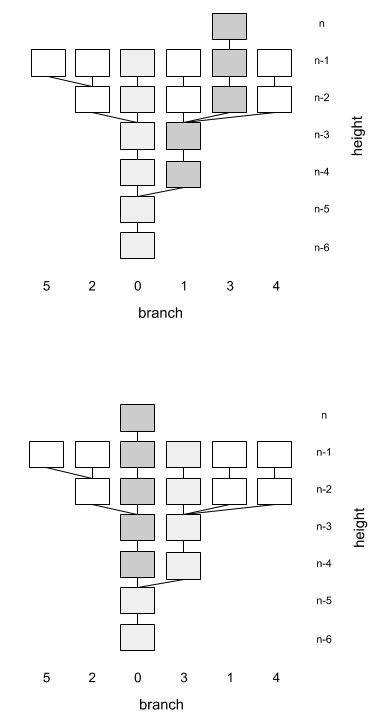
\includegraphics[width=1.00\linewidth]{branch_restructure3.png}
\subsection{Dynamic Hash Difficulty}
Hash difficulty adjustment is performed based on a simple moving average.  The network is configured so that target time \textit{v} is 10 minutes per block, difficulty adjustment span \textit{s} is 500, timestamp sample size \textit{n} is 2, and minimum hash difficulty \textit{m} is 1.  \textit{t} denotes the block's timestamp at height \textit{h}. \textit{d} denotes the present difficulty:
\begin{align*}
&Let\ {f} : (t,h)\mapsto \frac{t_h + t_{h-1} + \dots + t_{h-n}}{n+1} \\\\
&Let\ \Delta{t} = {f(t_h,h)} - {f(t_{h-s},h-s)}\\
\end{align*}
\[
d_h = 
\begin{cases}
	d_{h-1} & (h-2\leq s) \vee (\Delta{t} = v\cdot s)\\
	d_{h-1} + 1 & \Delta{t}<v\cdot s\\
	d_{h-1} - 1 & \Delta{t}>v\cdot s\\
\end{cases}
\]
By taking this approach, the block's hash difficulty can be calculated deterministically without the need to persist it in the block header.\\
Single timestamps are not a reliable metric as miners can populate the value arbitrarily. Therefore, we take the arithmetic mean $\bar{t}$ of $t_h$ and its \textit{n} previous \textit{t}'s:
\begin{align*}
\bar{t} = \frac{1}{n+1}\sum_{i=h-n}^{h} t_i
\end{align*}
\subsection{Network}
CrankChain takes a unique approach in the full node design by implementing a RESTful API over remote procedure calls.  Rest allows the CRUD operations necessary for the network to operate and pose no disadvantages over the latter.  In fact, interaction with the full nodes becomes simpler for web-based applications wishing to communicate with a node since HTTP verbs are already supported by clients.
**Publish/Subscribe models are used to broadcast messages across peers using \textit{ZeroMQ}.
\footnotetext[7]{future implementation}

\subsection{Mining}
Currently, CrankChain operates on a \textit{Proof-of-Work}\cite{conf:nakamoto} system.  In order to avoid centralization of mining, memory-hard slow hashes are preferred over pure computational fast hashes. \textit{Scrypt} was chosen as the hash algorithm.  Though it has received criticism for not being ASIC-resistant, this can be corrected by using \textit{Scrypt} with different factors.  Configurable \textit{Scrypt} factors according to \textit{(Scrypt---Wikipedia)}\cite{wiki:scrypt} include:
\begin{itemize}
\item \textit{Passphrase} - The string of characters to be hashed.
\item \textit{Salt} - A string of characters that modifies the hash to protect against Rainbow table attacks
\item \textit{N} - CPU/memory cost parameter.
\item \textit{p} - Parallelization parameter; a positive integer satisfying \textit{p} $\leq$ (2\textsuperscript{32}-1) * \textit{hLen / MFLen}.
\item \textit{dkLen} - Intended output length in octets of the derived key; a positive integer satisfying dkLen $\leq$ (2\textsuperscript{32}-1) * hLen.
\item \textit{r} - The blocksize parameter, which fine-tunes sequential memory read size and performance. 8 is commonly used.
\item \textit{hLen} - The length in octets of the hash function (32 for SHA256).
\item \textit{MFlen} - The length in octets of the output of the mixing function. Defined as \textit{r} * 128 in RFC7914.
\end{itemize}
CrankChain's Scrypt hash is configured with the following factors: \textit{N}=1024, \textit{r}=1, \textit{p}=1, \textit{dkLen}=32
\subsection{**Proof of Collaboration (proposal)}
\footnotetext[7]{future implementation}
\subsubsection{Pain point}
Proof of Work mining is essentially a race to find a nonce that yields the correct hash pattern. 
There are no guaranteed rewards, and the likelihood that a miner using standard hardware is able to compete with large mining operations is very low. A clear advantage exists for individuals with a) capital to invest in such operations and b) have access to free or inexpensive electricity. \\
Mining pools are still orchestrated by a single entity with mercenary computational resources.
This would not be a problem if the probability of being rewarded grew linear to one's hash rate. Nevertheless, one’s probability grows exponentially as their ability to compute hashes grows. A slower machine's probability of discovering a valid block diminishes as the qualifying nonce reaches higher numbers. The likelihood of a low nonce decreases as the hash difficulty increases. Since the network rewards a miner for discovering blocks quicker than the rest of the network, it opens up susceptibility to 51\% attacks\cite{btcwiki:weaknesses} while discouraging common folks from mining.\\
In essence, the system designed around decentralization can be inadvertently centralized. There is a valid argument that the reward of hijacking a PoW network would not outweigh the cost\cite{btcwiki:weaknesses}. On the other hand, cost may not be a hindrance to particular entities that may feel threatened by the existence of such a network.
\subsubsection{Goals}
\begin{itemize}
\item wider, evenly distributed network
\item linear relationship between block rewards and capital investment
\item linear relationship between block rewards and uptime
\item zero slope relationship between block rewards and hash time
\item reward uptime rather than hash rate
\item no centralization
\item no censorship
\end{itemize}
\subsubsection{Proposal}
The author proposes an alternative system to \textit{Proof-of-Work} known as \textit{Proof-of-Collaboration}.  The system adheres to the following protocol:
\paragraph{On-chain node registry}
\begin{enumerate}[noitemsep,nolistsep]
\item New node registers by transacting a fee to a collaborator registration address and \textit{REGISTRATION} transaction type. The transaction would include the host's address in the metadata.
\item Once the block containing the node registry transaction has reached finality, other collaborators acknowledge the new node.
\item If a collaborator is unable to reach another collaborator, it records downtime in its local peer database.
\item Collaborators are acknowledged in ascending order by the locally recorded downtime. The greatest advantage goes to the collaborators with the least recorded downtimes which are guaranteed to partake in the mining of every block
\end{enumerate}

\paragraph{Collaborative mining}
\footnotetext[1]{this step may not be necessary}
By following this protocol, the chain effectively eliminates miners competing for a block.  This also means:
\begin{enumerate}[noitemsep]
\item Collaborators take turns initiating the mining process by its registration transaction's block height.  When it is a collaborator's turn to initiate the mining of a block, it starts by creating a block. *It may be the case that any collaborator can initiate the mining of a new block.
\item The collaborator calculates the merkle tree based on the included transaction hashes plus the coinbase transaction, and hashes it once (with the starting nonce, 0).
\item If the block pattern does not fit, it forwards the block header to a subset of registered collaborators sorted by ascending downtime. 
\item The next set of collaborators adds its own coinbase transaction repeats the previous two steps.
\item If the block pattern fits the chain, it broadcasts the block to all nodes.
\item If the block pattern does not fit, and all registered collaborators were exhausted, the nonce is incremented by 1 and repeated *It may be the case that simply changing the order of contributing collaborators will provide enough permutations of the merkel tree that the block pattern may be satisfied.
\[{n}_{Pr} = \frac{n!}{(n-r)!}\]
\item Block rewards are divided among contributing collaborators.
\end{enumerate}
\begin{itemize}[noitemsep]
\item The block header must store additional information: transactions index and coinbase addresses. 
\item Hash difficulty does not need to increase due to the nature of this system
\item Each block will involve a varying number of nodes, thus varying reward amounts
\item Registry transactions should cost a small fee in coins so that nodes don’t register and go offline without being penalized
\item Network stability is more important than computational power
\item Cost/reward is linearly correlated and encourages more users to contribute to the network
\end{itemize}

Coinbase transaction fees are calculated:
\[Let\ {C} = \{col_1,col_2,\dots,col_n\}\]
\[{fee}=\frac{reward}{|C|}\]

\paragraph{Attack vectors}
Sybil attacks are currently the greatest concern for Proof of Collaboration.  A malicious actor may attempt to register a large number of collaborators and hash every permutation of the actors' own node addresses until the block hash satisfies the hash difficulty pattern.  There are a few strategies to mitigate this to some degree:
\begin{enumerate}[noitemsep]
\item Restrict IPs based on CIDR block.
\item Disallow incrementing the nonce completely
\item Adjust hash difficulty based on the number of registrants
\item Enforce a certain order based on registration block height
\item Passing a bloom filter?
\item Chain of verifiable signatures?
\[S_{priv_C}(S_{priv_B}(S_{priv_A}(hash))) = {validhash}\]
\[V_{pub_A}(V_{pub_B}(V_{pub_C}(validhash))) = {hash}\]
\end{enumerate}


\section{System Overview}
\subsection{Scaling}
The network largely follows the traditional single dimensional blockchain design as transaction speed is less of a concern than durability and security.  The author does not believe \textit{Bitcoin} to have a scaling issue\cite{wiki:btcscalability}, but a performance issue.  The network's bandwidth is very limited, but the mempool acts as an effective rate limiter and priority queue based on transaction fees.\\
In order for CrankChain to be resilient to large volumes of transactions, each node must be able to withstand a reasonable amount of inbound requests.  We achieve this by separating the resource heavy requests from the lighter requests and routing the heavier requests to a queue.  Queue consumers are loosely coupled and can be scaled to a configurable number of processes optimal for that particular node's hardware.  Meanwhile, light resource requests can fetch data directly or optionally via cache.  Costly request endpoints are also permissioned to known connected peers.\\
The mempool transactions are persisted to physical store and deleted when they are mined.  This offers a few advantages over traditional in-memory mempools.  The most important advantage is the fact that separate processes can access the same data without relying on an interprocess pipe.\\
Miners are also a separate process which can be enabled/disabled independently from the rest of the node.
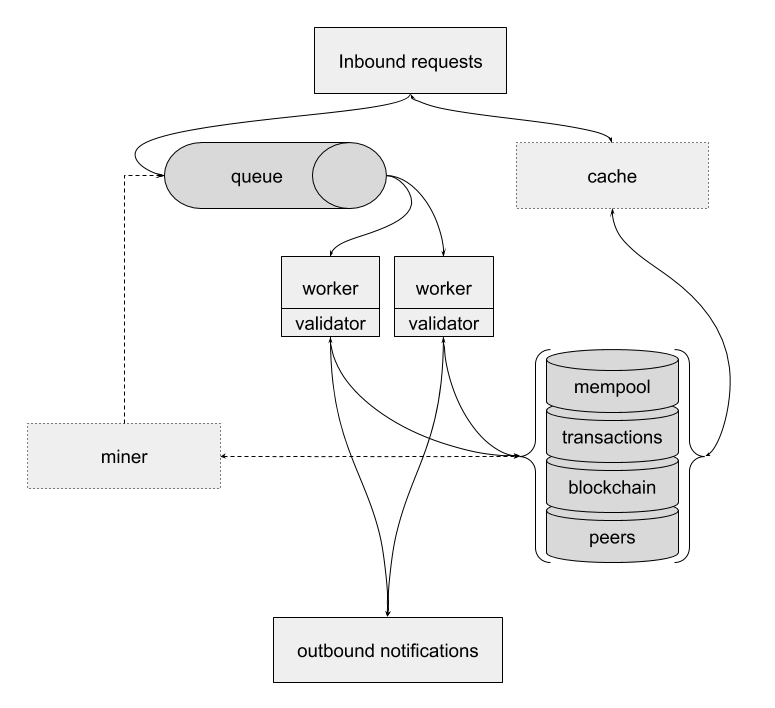
\includegraphics[width=1.00\linewidth]{node_design.png}
\subsection{Persistence}
CrankChain uses SQLite for persistence.  SQLite possesses several properties that make it ideal as the underlying datastore.  It is fast, process-safe, thread-safe, resilient to file corruption, and it does not require a separate standalone instance.  In addition, it includes an advanced query language, context manager for transactions, and built-in locking.  Python requires multiprocessing over threads to achieve performance gain.  LevelDB was considered due to its superiority in performance, but it is not process-safe and susceptible to file corruption.
\subsection{Queueing}
CrankChain relies heavily on the queue to regulate the inflow of requests that require validation and database write operations.  A light whitelist validation is all that occurs upfront to provide a synchronous acceptance or rejection response before the message is enqueued.\\
The queue process is a \textit{ZeroMQ} push/pull proxy bound to a local UNIX socket.  \textit{ZeroMQ} is a brokerless messaging queue, but the proxy acts as a simple broker\cite{website:zeromqguide}.\\
**The notification process is a \textit{ZeroMQ} publisher that is TCP bound.\\
**The listener process is a \textit{ZeroMQ} subscriber that is also TCP bound.
\footnotetext[7]{future implementation}
\subsection{Processes and Threads}
A major architectural objective is horizontal scalability.  Implementation in Python adds challenges in concurrent operations due to the nature of the global interpreter lock.  Since Python is not especially known for its benchmarking performance, relying on threads to increase speed is less than ideal.  A better approach is to spawn separate processes or deployments as needed.  The downside to running multiple processes is the lack of a shared memory space; communication between processes must rely on an interprocess pipe or queue.  CrankChain dedicates a process for the API layer, a process for the queue, and a configurable number of processes for the queue processors.  The API layer is a thin \textit{Bottle} process which merges public and permissioned endpoints and routes them to the appropriate service or queue.  The queue process independently runs the \textit{ZeroMQ} proxy which acts as a messaging broker.  Each of the producers and consumers communicate to the broker via a local UNIX socket which makes it interprocess compatible.  Consumer processes have the majority of the responsibilities as it validates, persists, and notifies.  While the consumer processes can be scaled to an arbitrarily high number, node operators should be cautious as to not overwhelm the database with excessive write operations as SQLite does not allow concurrent writes.\\  
Finally, the miner is a separate module that runs independently of the node.  It communicates with the queue and the database.  It should use the optional C compiled module for a more desirable hash rate.\\
**The notification process runs a \textit{ZeroMQ} publishing server for broadcasting outbound notifications.  Consumers of this queue are external.\\
**The listener process runs a \textit{ZeroMQ} subscriber for listening to its external peer subscriptions for inbound notifications.
\footnotetext[7]{future implementation}
\subsection{Caching}
Caching is optional but encouraged.  CrankChain does not natively provide caching, but is trivial to integrate any number of available standalone caching services such as Memcached or Redis.  


\section{Attack Vectors}
\subsection{Double-spend Attack}
CrankChain nodes will calculate account balances (when queried) rather than seek the last known transaction and return the UTXO (\textit{Bitcoin}).  CrankChain has the luxury of doing this because it uses a less primitive data store with indexed public addresses for a \textit{O(1)} random access lookup.  UTXO does, however, provide another purpose---prevent double-spend attacks\cite{conf:nakamoto}.  During each transaction, the entire balance of the wallet is spent before it is returned upon completion.  Concurrent transactions cannot occur.  \textit{Ethereum} follows a different strategy to mitigate double-spend attacks---include an incrementing nonce with each transaction\cite{whitepaper:buterin}.  A transaction that does not include a nonce with the correct sequence is invalid.\\
CrankChain follows neither strategy and requires transactions to include a hash of the previous transaction, similar to blocks.  Effectively, each public address forms a mini-chain of transactions which prove undeniably, that one transaction follows the next.  Since transaction hashes are guaranteed to be unique (per branch), duplicate transaction hashes, ie transactions of the same amount, to the same recipient, with the exact same timestamp are \textbf{not} allowed.
\subsection{DDOS Attack}
While no public service is completely resistant to DDOS attacks, certain measures are taken.  In order to mitigate DDOS attacks from unknown hosts, POST transaction endpoints (from light clients) and light GET request endpoints will be the only endpoints available to the public.  Costlier calls will be restricted to known peers or dropped with a 403.  Known peers must go through a prior handshake/verification.  In order to mitigate DDOS attacks from known peers, a few measures are taken.  First, a maximum number of peers is allowed and configurable per node.  Second, costly POST requests will be asynchronously placed on a queue before validation/processing take place on one of the queue consumer processes which is also configurable per node.  Optionally, a caching layer can be added behind.  The Python implementation of CrankChain uses \textit{Bottle}\cite{website:bottledocs} which ships with adapters to common WSGI servers.  It may also be beneficial for each node to operate behind an NGINX reverse proxy with rate limiting enabled.  
\paragraph{Spam Attack}
Transaction fees and the previous transaction hash requirement prevent a user from spamming the network with an excessive number of blocks.  It is relatively cheap for a node to filter out invalid transactions from entering the mempool.  A random access \textit{O(1)} lookup is all that is necessary to drop such transactions.  If a transaction isn't finalized, its hash does not qualify as the subsequent transaction's previous hash.\\
Proof-of-Work prevents a miner from spamming the network with an excessive number of blocks.  Such an attack would require a hash rate much higher than the rest of the network.  If the attacker invested in the resources capable of performing a spam attack, it would be short-lived due to the adjustable hash rate.  
\paragraph{Chain Death Spiral}
A \textit{Chain Death Spiral} occurs when a network faces a sudden loss of mining power, causing the targeted block rate to be missed.  This weakness was witnessed on \textit{Bitcoin} Cash when its blocktime reached 15 hours, prompting it to hard fork and apply an \textit{Emergency Difficulty Adjustment} to relax the difficulty sooner than scheduled\cite{website:btcandblockchain}.
If an attacker with a dominant hash rate decides to cease mining CrankChain, a \textit{Chain Death Spiral} should not pose a threat due to CrankChain's \textit{dynamic hash difficulty adjustment}.  The hash difficulty is recalculated every block in a deterministic fashion using moving averages and may adjust either way.

\subsection{Replay Attack}
Like many other blockchains, replay attacks are prevented by prefixed wallet addresses\cite{btcwiki:addressprefixes}.  CrankChain mainnet will be prefixed with \textit{m} while testnet addresses will be prefixed with \textit{t}
\subsection{Sybil Attack}
Sybil attacks are also mitigated in a similar fashion to other networks.  By restricting IPs based on CIDR block, CrankChain makes it difficult to perform this attack.  \textit{Bitcoin} also takes this approach by restricting nodes from establishing an outbound connection to more than one IP address per /16 (x.y.0.0)\cite{btcwiki:weaknesses}.
\subsection{Quantum Attack}
If quantum computing resources become available and threatens the current cryptosystems in play, CrankChain can simply upgrade to quantum resistant cryptosystems and allow users to migrate their wallets


\section{Conclusion}
In conclusion, the author has presented implementation details surrounding CrankChain.  In doing so, it was proven that decentralized asset registration, tokenization, and exchange can be achieved without added complexity, smart contracts, nor compromised decentralization.  Furthermore, a scalable implementation was built using Python, a language not known for performance.  \\
The author has also proposed a new mining mechanism known as \textit{Proof of Collaboration} or \textit{PoC} with hopes that the protocol will mature and eventually be implemented into CrankChain and other future blockchains.\\\\
\textit{CrankChain was first introduced as Cranky Coin on cranklin.com, 2017}\cite{website:cranklincrankycoin}
\clearpage
\bibliography{references}
\bibliographystyle{plain}
\end{document}